\newcommand*{\TemplatePath}{../../../template/slides}
\newcommand*{\SourcesPath}{../../../sources}
\newcommand*{\ImagePath}{../../../images}
\newenvironment{fig}[1]
{
	\def\tempone{#1}
	% \vspace{#2}
	\begin{center}
		}
		{
		Abb. \arabic{secnum}.\arabic{fignum}: \tempone
	\end{center}
	\stepcounter{fignum}
}
   
\newcommand{\framehead}[1]{
	\frametitle{#1}
	\section{#1}
}
   
\newcommand{\framesubhead}[1]{
	\frametitle{#1}
	\subsection{#1}
}

\newcommand{\headerframe}[1]{
	\begin{frame}

		\section{#1}
		\begin{center}
			\Huge{#1}
		\end{center}
	
	\end{frame}
}

\newcommand{\headerframealias}[2]{
	\begin{frame}

		\section{#2}
		\begin{center}
			\Huge{#1}
		\end{center}
	
	\end{frame}
}

\newcommand{\headerframelight}[1]{
	\begin{frame}

		\begin{center}
			\Huge{#1}
		\end{center}
	
	\end{frame}
}



\newcommand*{\tbd}[1]{
	\colorbox{red}{{\color{white}\textbf{TBD}}} {\color{red}#1} \\
}
\newcommand*{\tbditemlabel}{
	\colorbox{red}{{\color{white}\textbf{TBD}}} \\
}
\newenvironment{todolist}
{\begin{itemize}[label=\tbditemlabel,leftmargin=36pt]
		}
		{
	\end{itemize}
}

\newcommand*{\boxitemlabel}{
	\colorbox{primary}{{\color{primaryText}\textbf{\textsf{\theenumi}}}}
}

\newcommand*{\boxitem}[1]{
	\colorbox{primary}{{\color{primaryText}\textbf{\textsf{#1}}}}
}

% \newcommand*{\chevron}{
%   \colorbox{MaterialDeepPurple500}{{\color{white}\textbf{\textsf{\faIcon{caret-right}}}}}
% }
\newcommand*{\chevron}{
	\faIcon[regular]{long-arrow-alt-right}
}

\newenvironment{hints}
{\begin{itemize}[label=\chevron,leftmargin=18pt]
		}
		{
	\end{itemize}
}

\newcommand*{\checkitemlabel}{
	\faIcon[regular]{check-square}
}
\newenvironment{checklist}
{\begin{itemize}[label=\checkitemlabel,leftmargin=18pt]
		}
		{
	\end{itemize}
}

\newcommand*{\uncheckitemlabel}{
	\faIcon[regular]{square}
}
\newenvironment{unchecklist}
{\begin{itemize}[label=\uncheckitemlabel,leftmargin=18pt]
		}
		{
	\end{itemize}
}

\newcommand*{\hint}{\item}

\newenvironment{steps}
{\begin{enumerate}[label=\boxitemlabel]
		}
		{
	\end{enumerate}
}

\newcommand*{\itembox}[1]{\colorbox{MaterialDeepPurple500}{{\color{white}\textbf{\textsf{#1}}}}}

\newcommand*{\lineitemlabel}{
	Zeile \colorbox{MaterialDeepPurple500}{{\color{white}\textbf{\textsf{\theenumi}}}}
}


\newcommand\crule[3][black]{\textcolor{#1}{\rule{#2}{#3}}}


\newcommand*{\taskitemlabel}[1]{
	\colorbox{black}{{\color{white}\faIcon{pen-square}~\textbf{\textsf{#1}}}}
}

% !TEX root = ../../skript.tex

\documentclass[a4paper, oneside, titlepage, 11pt, hidelinks]{report}

\renewcommand{\familydefault}{\sfdefault}

\usepackage{geometry}
\geometry{
	a4paper,
	width=13cm,
	left=3cm,
	bottom=2cm,
  top=2cm,
  marginparsep=0.5cm,
  marginparwidth=4.6cm,
}

\usepackage[ngerman]{babel}
\usepackage{blindtext}
\usepackage{graphicx}
\usepackage{float}
\usepackage{tabularx}
\usepackage[labelsep=space]{caption}

\usepackage{csquotes}
\usepackage[backend=biber, refsegment=chapter, defernumbers=true, style=apa]{biblatex}

\usepackage{xcolor}
\definecolor{bb}{RGB}{0,138,217}
% \definecolor{purple100}{RGB}{209,196,233}
\usepackage{xcolor-material}
% \definecolor{MaterialDeepPurple50}{RGB}{237,231,246}

\usepackage{cloze}
\clozesetfont{\ttfamily\Large}
\clozeset{
	textcolor=bb,
	align=center,
	% margin=1cm,
}
\clozehide

\usepackage[inline,shortlabels]{enumitem}

\setlength{\parindent}{0pt}
\setlength{\parskip}{0.5em}
\setlength{\abovecaptionskip}{3pt}
% \linespread{1.6}

\usepackage{setspace}

\usepackage{titling}

\usepackage{minitoc}
\renewcommand{\mtctitle}{Inhaltsverzeichnis}
\renewcommand{\mtifont}{\large\sffamily}
\renewcommand{\mtcfont}{\small\sffamily}
\renewcommand{\mtcSfont}{\small\sffamily}
\renewcommand{\mtcSSfont}{\small\sffamily}
\renewcommand{\mtcSSSfont}{\small\sffamily}

\usepackage{fontspec}
\usepackage[pro]{fontawesome5}
\usepackage[many]{tcolorbox}
% Hint box
\newtcolorbox{hintbox}[1][]{
	arc=0pt,
  breakable,
  freelance,
  colback=primary100,
  colbacktitle=primary300,
	fonttitle=\bfseries,
	fontupper=\sffamily,
  bottomrule=8pt,
	boxrule=0pt,
  colframe=white,
  overlay unbroken and first={
  \draw[primary,line width=3pt]
    (frame.north west) -- 
    (frame.south west);
  },
}
% Hint box
\newtcolorbox{hintbox*}[1][]{
	arc=0pt,
	toptitle=5pt,
	bottomtitle=5pt,
  breakable,
  freelance,
  title=\faIcon{box-open}~#1,
  colback=primary100,
  colbacktitle=primary300,
  coltitle=primaryText,
	fonttitle=\bfseries,
	fontupper=\sffamily,
  bottomrule=8pt,
	boxrule=0pt,
  colframe=white,
  overlay unbroken and first={
  \draw[primary,line width=3pt]
    (frame.north west) -- 
    (frame.south west);
  },
}


\usepackage{listings}
\lstset{
    basicstyle=\footnotesize\ttfamily,
    numbers=left,
    stepnumber=1,
    showstringspaces=false,
    tabsize=2,
    breaklines=true,
		breakatwhitespace=false,
		frame=leftline,
		aboveskip=00pt,
    keywordstyle=\bf,
    escapeinside={(*}{*)}
}

\usepackage{dirtree}

\usepackage{marginnote}

\usepackage{hyperref}

\usepackage{pdflscape}

\usepackage[os=win]{menukeys}
\renewmenumacro{\directory}{pathswithfolder}


\title{Lecture Title\\\vspace{0.5cm}\textit{Akronym}\\\vspace{0.5cm}{\small\textit{v1.0.0}}}
\date{WS 1988}
\author{Author \\ \texttt{abc@domain.tld}}


\addbibresource{sources.bib}
\subtitle{Kapitel 1: Einführung}
   
\begin{document}

\frame{\titlepage}

\headerframe{Organisatorisches}

\begin{frame}
	\frametitle{Folien \& Materialien}

	\begin{center}
		\url{https://abc.domain.tld/}
	\end{center}
\end{frame}


\begin{frame}
	\frametitle{Inhaltliche Ausrichtung}

	\begin{figure}
		\centering
		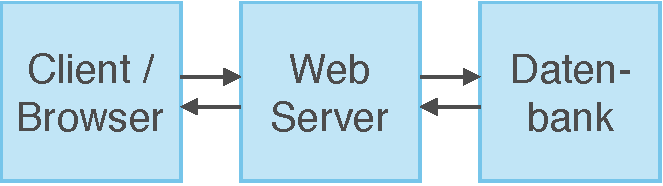
\includegraphics[width=1.0\textwidth]{\ImagePath/system_map}
	\end{figure}
\end{frame}

\begin{frame}
	\frametitle{Inhaltliche Ausrichtung}
	\begin{columns}
		\begin{column}{0.5\textwidth}
			\begin{figure}
				\centering
				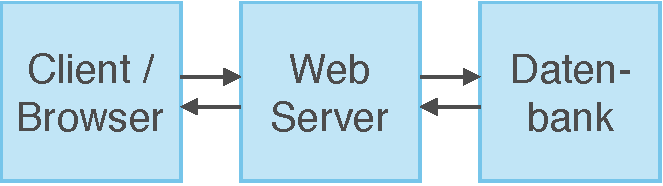
\includegraphics[width=1.0\textwidth]{\ImagePath/system_map}
			\end{figure}
		\end{column}
		\begin{column}{0.5\textwidth}
			\begin{hints}
				\item X
				\item Y
			\end{hints}
		\end{column}
	\end{columns}
\end{frame}


\headerframe{Neue Sektion}

\begin{frame}
	\frametitle{Neue Sektion}
	\begin{columns}
		\begin{column}{0.5\textwidth}
			\begin{figure}
				\centering
				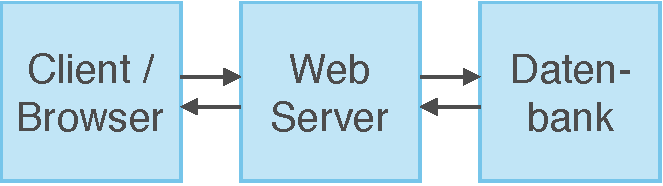
\includegraphics[width=1.0\textwidth]{\ImagePath/system_map}
			\end{figure}
		\end{column}
		\begin{column}{0.5\textwidth}
			\begin{steps}
				\item X
				\item Y
			\end{steps}
		\end{column}
	\end{columns}
\end{frame}

\headerframelight{Neue Sektion ohne }

\begin{frame}
	\frametitle{Neue Sektion ohne Section}
	\begin{columns}
		\begin{column}{0.5\textwidth}
			\begin{figure}
				\centering
				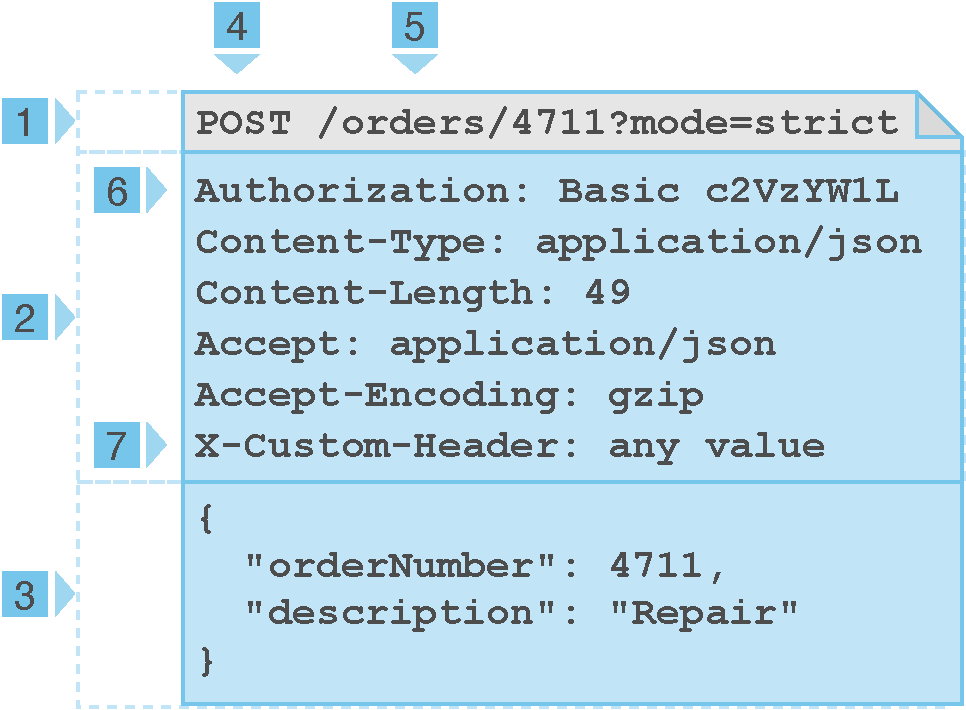
\includegraphics[width=1.0\textwidth]{\ImagePath/sample/http_message}
			\end{figure}
		\end{column}
		\begin{column}{0.5\textwidth}
			\begin{steps}
				\item A
				\item B
			\end{steps}
		\end{column}
	\end{columns}
\end{frame}

\headerframealias{Neue Sektion}{mit Alias}

\begin{frame}
	\frametitle{Neue Sektion mit Alias}
	\begin{columns}
		\begin{column}{0.5\textwidth}
			\begin{figure}
				\centering
				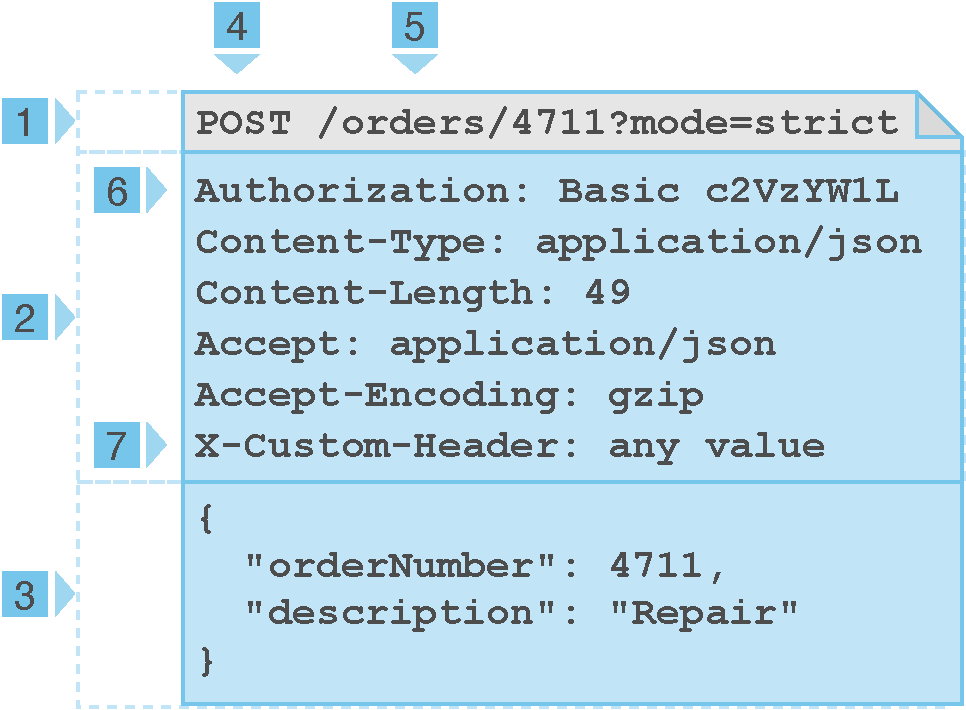
\includegraphics[width=1.0\textwidth]{\ImagePath/sample/http_message}
			\end{figure}
		\end{column}
		\begin{column}{0.5\textwidth}
			\begin{steps}
				\item M
				\item N
			\end{steps}
		\end{column}
	\end{columns}
\end{frame}


% !TEX root = ../../skript.tex

% \bibliographystyle{apacite}
% \printbibliography[segment=2,heading=subbibliography]
% \nocite{*}

\end{document}